% T12 C/D, chapitre 11 : Statistiques. Source : le livre « Terminales scientifiques » (Stat/Lesona, Stat/Exo).
% Les exercices tirés d’autres ouvrages ne sont pas repris (décision du 2 novembre 2026).

\TCDLessonStyleOn
\chapter{Statistiques}
      \section{S\'eries statistiques \`a une variable}
            \begin{defi}
                  Consid\'erons le tableau suivant qui donne les \^ages des \'etudiants d'une classe
                  de terminale comptant 43 \'el\`eves : \newline
                  \begin{tabular}{|c|c|c|c|c|c|c|}
                        \hline
                        Ages                   & 15 & 16 & 17 & 18 & 19 & 20 \\
                        \hline
                        Nombre d'\'el\`eves    &  2 &  6 & 17 & 14 &  3 &  1 \\
                        \hline
                  \end{tabular}
                  %
                  \begin{description}
                        \item L'ensemble des 43 \'el\`eves constitue la \emph{population statistique}.
\index{Population}
                        \item Chaque \'el\`eve est un \emph{individu} ou \emph{unit\'e statistique}.
\index{Individu}
\index{Unite@Unit\'e}
                        \item Le \emph{caract\`ere statistique} \'etudi\'e dans ce tableau est l'\^age.
\index{Caractere@Caract\`ere}
                        \item Il s'agit d'un \emph{caract\`ere quantitatif}, c'est-\`a-dire qu'il peut s'exprimer en nombre.
                              Un caract\`ere qui ne peut pas s'exprimer en nombre est dit \emph{qualitatif}.
\index{Caractere@Caract\`ere!quantitatif}
\index{Caractere@Caract\`ere!qualitatif}
                        \item Le caract\`ere \'etudi\'e ici prend un nombre fini de valeurs, on dit qu'il est \emph{discret}.
\index{Caractere@Caract\`ere!discret}
                              Un caract\`ere qui peut prendre n'importe quelle valeur r\'eel dans un intervalle 
\index{Caractere@Caract\`ere!continu}
                              est dit \emph{continu}.
                        \item Un caract\`ere quantitatif est aussi appel\'e \emph{variable}.
\index{Variable}
                        \item Pour \'etudier une variable continue, on partage l'intervalle dans lequel elle prend valeurs en 
\index{classe}
                              un nombre fini d'intervalle qu'on appelle \emph{classe}.
                        \item Les \emph{modalit\'es} d'une variable discr\`ete sont les valeurs que peut prendre la variable.
\index{Modalite@Modalit\'e}
                        \item L'\emph{effectif} d'une modalit\'e est le nombre d'individus pr\'esentant cette modalit\'e.
\index{Effectif}
                        \item La \emph{fr\'equence} d'une modalit\'e est le 
\index{Frequence@Fr\'equence}
                              rapport entre l'effectif de cette modalit\'e et l'effectif total.
                        \item Dans le cadre d'une variable quantitative, l'\emph{effectif cumul\'e}
\index{Effectif!cumule@cumul\'e}
                              d'une modalit\'e $a$ est la somme des effectifs des modalit\'es inf\'erieures ou \'egales \`a $a$.
                              De m\^eme, la \emph{fr\'equence cumul\'ee} d'une modalit\'e $a$ est la somme des fr\'equences
\index{Frequence@Fr\'equence!cumule@cumul\'e}
                              des modalit\'es inf\'erieures ou \'egales \`a $a$.
                  \end{description}
                  %
                  \begin{ex}
                        On donne la s\'erie statistique du 
                        nombre de fr\`eres et s\oe urs des \'etudiants d'une classe de terminale :
                        \begin{tabular}{cccccccccc}
                              1 & 2 & 0 & 1 & 1 & 0 & 2 & 3 & 2 & 3 \\
                              3 & 0 & 4 & 1 & 2 & 2 & 4 & 2 & 0 & 3 \\
                              1 & 2 & 0 & 2 & 5 & 1 & 2 & 2 & 3 & 0 
                        \end{tabular}
                        Ces donn\'ees peuvent \^etre repr\'esent\'ees de mani\`ere plus organis\'ee par le tableau suivant :\newline
                        \begin{table}[H]
                        \centering
                        \begin{tabular}{c|c|c|c|c}
                        Valeur   & Effectif & Fr\'equence & Effectifs & Fr\'equence \\
                        ($x_i$)  & ($n_i$)  &  ($f_i$)    & cumul\'es &  cumul\'es  \\
                        \hline
                              0        &       6          &       0,2           &       6             &         0,2           \\
                              1        &       6          &       0,2           &      12             &         0,4           \\
                              2        &      10          &       0,33          &      22             &         0,73          \\
                              3        &       5          &       0,17          &      27             &         0,90          \\
                              4        &       4          &       0,07          &      29             &         0,97          \\
                              5        &       1          &       0,03          &      30             &         1,0           \\
                        \end{tabular}
                        \caption{Tableau repr\'esentant le
                                 nombre de fr\`eres et s\oe urs des \'etudiants d'une classe de terminale.}
                        \label{tab:variable discret}
                        \end{table}
                  \end{ex}
            \end{defi}
            %
            \subsection{Repr\'esentation graphique}
                  Il est souvent pr\'ef\'erable de visualiser les donn\'ees par une repr\'esentation graphique.
                  %
                  \subsubsection{Diagramme en b\^atons}
\index{Diagramme!en batons@en b\^atons}
                        Les diagrammes en b\^atons sont utilis\'es pour repr\'esenter des variables discr\`etes.
                        La s\'erie statistique pr\'ec\'edente peut par exemple \^etre 
                        repr\'esent\'e par un diagramme en b\^atons (Figure~\ref{fig:diagramme en batons}).
                        %
                        \begin{figure}%[H]
                              \centering
                              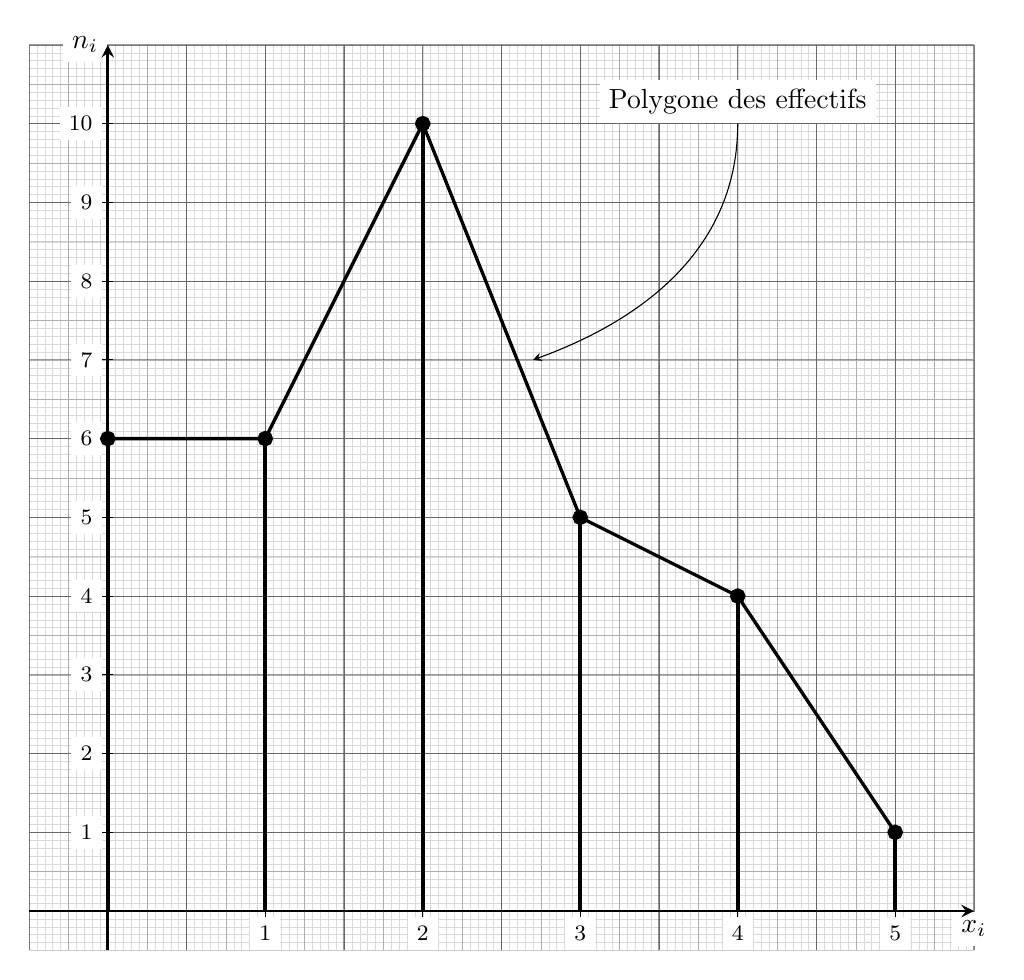
\begin{tikzpicture}[>=stealth,x=2.0cm,y=1.0cm,ybar,ycomb]
                                    \draw [color=black, xstep=1.0cm,ystep=1.0cm, line width=.4pt, opacity=.4] 
                                          (-0.5,-0.5) grid (5.5,11);
                                    \draw [color=black, xstep=0.5cm,ystep=0.5cm, line width=.2pt, opacity=.2] 
                                          (-0.5,-0.5) grid (5.5,11);
                                    \draw [color=black, xstep=0.1cm,ystep=0.1cm, line width=.15pt, opacity=.15] 
                                          (-0.5,-0.5) grid (5.5,11);
                                    \draw[] (0,11) node[fill=white, left] {$n_i$};
                                    \draw[] (5.5,0) node[fill=white, below] {$x_i$};
                                    \draw[->,color=black, line width=1pt] (-0.5,0) -- (5.5,0);
                                    \foreach \x in {1,2,...,5}
                                    \draw[shift={(\x,0)},color=black] (0pt,2pt) -- (0pt,-2pt) 
                                          node[below,fill=white] {\footnotesize $\x$};
                                    \draw[->,color=black, line width=1pt] (0,-0.5) -- (0,11);
                                    \foreach \y in {1,2,...,10}
                                    \draw[shift={(0,\y)},color=black] (2pt,0pt) -- (-2pt,0pt) 
                                          node[left,fill=white] {\footnotesize $\y$};
                                    \draw[ultra thick]
                                          plot[ycomb,thin,mark=*] coordinates{(0,6) (1,6) (2,10) (3,5) (4,4) (5,1)};
                                    \draw[very thick] (0,6) -- (1,6) -- (2,10) -- (3,5) -- (4,4) -- (5,1);
                                    \draw[] (4,10) node[fill=white, above] {Polygone des effectifs};
                                    \draw[->] (4,10) to[out=-90,in=20] (2.7,7);
                              \end{tikzpicture}
                              \caption{Diagramme en b\^atons repr\'esentant le tableau~\ref{tab:variable discret}.}
                              \label{fig:diagramme en batons}
                        \end{figure}
                  %
                  \subsubsection{Histogramme}
\index{Histogramme}
                        Consid\'erons le tableau~\ref{tab:variable continue}.
                        On a regroup\'e les donn\'ees par classe d'amplitude 5~cm. \newline
                        \begin{table}[h!]
                        \centering
                              \begin{tabular}{|c|c|c|}
                              \hline
                              Classes       & Effectifs    & Centre  \\
                              \hline
                              [150 ; 155[   &       2      &  152.5  \\
                              \hline
                              [155 ; 160[   &       4      &  157.5  \\
                              \hline
                              [160 ; 165[   &       5      &  162.5  \\
                              \hline
                              [165 ; 170[   &       8      &  167.5  \\
                              \hline
                              [170 ; 175[   &       4      &  172.5  \\
                              \hline
                              [175 ; 180[   &       3      &  177.5  \\
                              \hline
                              [180 ; 185[   &       2      &  182.5  \\
                              \hline
                              [185 ; 190[   &       1      &  187.5  \\
                              \hline
                              \end{tabular}
                        \caption{Tableau pr\'esentant les tailles en centim\`etres des \'el\`eves d'une classe de terminale.}
                        \label{tab:variable continue}
                        \end{table}
                        %
                        Cette s\'erie peut \^etre repr\'esent\'ee graphiquement par le diagramme~\ref{fig:histogramme}.
                        %
                        \begin{figure}%[h!]
                        \centering
                              \begin{tikzpicture}[>=stealth,x=1.0cm,y=1.0cm,ybar interval]
                                    \draw [color=black, xstep=1.0cm,ystep=1.0cm, line width=.4pt, opacity=.4] 
                                          (-0.5,-0.5) grid (10,9.5);
                                    \draw [color=black, xstep=0.5cm,ystep=0.5cm, line width=.2pt, opacity=.2] 
                                          (-0.5,-0.5) grid (10,9.5);
                                    \draw [color=black, xstep=0.1cm,ystep=0.1cm, line width=.15pt, opacity=.15] 
                                          (-0.5,-0.5) grid (10,9.5);
                                    \draw[] (0,9.5) node[fill=white, left] {$n_i$};
                                    \draw[] (10,0) node[fill=white, below] {$x_i$};
                                    \draw[->,color=black, line width=1pt] (-0.5,0) -- (10,0);
                                    \foreach \x/\xtext in {1/150,2/155,3/160,4/165,5/170,6/175,7/180,8/185,9/190}
                                    \draw[shift={(\x,0)},color=black] (0pt,2pt) -- (0pt,-2pt) 
                                          node[below,fill=white] {\footnotesize \rotatebox{90}{$\xtext$}};
                                    \draw[->,color=black, line width=1pt] (0,-0.5) -- (0,9.5);
                                    \foreach \y in {1,2,...,8}
                                    \draw[shift={(0,\y)},color=black] (2pt,0pt) -- (-2pt,0pt) 
                                          node[left,fill=white] {\footnotesize $\y$};
                                    \draw[color=loko2!50!black,fill=loko1!80,fill opacity=.5, ultra thick]
                                          plot coordinates{(1,2) (2,4) (3,5) (4,8) (5,4) (6,3) (7,2) (8,1) (9,1)};
                                    \draw[ultra thick]
                                          (1.5,2) -- (2.5,4) -- (3.5,5) -- (4.5,8) -- (5.5,4) 
                                                  -- (6.5,3) -- (7.5,2) -- (8.5,1);
                                    \foreach \x/\y in {1.5/2,2.5/4,3.5/5,4.5/8,5.5/4,6.5/3,7.5/2,8.5/1}
                                          \filldraw (\x,\y) circle (2pt);
                                    \draw[] (8,8) node[fill=white, above] {Polygone des effectifs};
                                    \draw[->] (8,8) to[out=-90,in=20] (5.5,5);
                              \end{tikzpicture}
                              \caption{Histogramme repr\'esentant la s\'erie statistique de 
                                       la table~\ref{tab:variable continue}}
                              \label{fig:histogramme}
                        \end{figure}
                        \nota{
                              Dans un histogramme, 
                              il est souvent pr\'ef\'erable de travailler avec des classes d'amplitudes constantes.
                              Dans le cas o\`u les amplitudes des classes sont diff\'erentes,
                              l'effectif doit \^etre proportionnel \`a l'aire (et non \`a la hauteur).
                        }
                  %
                  \subsubsection{Diagramme en secteur}
\index{Diagramme!en secteur}                  
                        Le tableau~\ref{tab:religions} indique les religions les plus pratiqu\'ees
                        ainsi que le nombre de pratiquants en 2010.
                        
                        \begin{table}[h!]
                        \centering
                              \begin{tabular}{|c|c|c|c|}
                              \hline 
                              Religions & Nombre de   & Pourcentages & Angle du secteur \\ 
                                        & pratiquants &              &  correspondant   \\
                              \hline 
                              Christianisme & 2\,420 & 36,24 & 130,5 \\ 
                              \hline 
                              Islam & 1\,800 & 26,95 & 97,04 \\ 
                              \hline 
                              Sans religion & 1\,150 & 17,22 & 61,99 \\ 
                              \hline 
                              Hindouisme & 520 & 7,79 & 28 \\ 
                              \hline 
                              Bouddhisme & 400 & 5,99 & 21,56 \\ 
                              \hline 
                              Autres & 388 & 5,81 & 20,92 \\ 
                              \hline 
                              \end{tabular} 
                              \caption{Tableau indiquant les religions les plus pratiqu\'es 
                                       ainsi que le nombre de pratiquants (en millions) en 2010.}
                              \label{tab:religions}
                        \end{table}
                        %
                        Ce tableau peut \^etre repr\'esent\'e par un diagramme en secteur 
                        comme dans la figure~\ref{fig:religions}.
                        \begin{figure}[H]
                        \centering
                              \begin{tikzpicture}[scale=4.5]
                                    \draw[very thick] (0,0) circle (1);
                                    \filldraw[fill=white] (0,0) -- (1,0) arc (0:130.5:1) -- cycle ; 
                                    \filldraw[fill=loko1] (0,0) -- (130.5:1) arc (130.5:227.49:1) -- cycle ; 
                                    \filldraw[fill=black] (0,0) -- (227.49:1) arc (227.49:289.49:1) -- cycle ; 
                                    \filldraw[fill=loko3] (0,0) -- (289.49:1) arc (289.49:317.52:1) -- cycle ; 
                                    \filldraw[fill=loko1!50!loko5] (0,0) -- (317.52:1) arc (317.52:339.08:1) -- cycle ; 
                                    \filldraw[fill=loko6] (0,0) -- (339.08:1) arc (339.08:360:1) -- cycle ; 
                                    \draw[black] ( 65:.55) node{Christianisme};
                                    \draw[white] (190:.60) node{Islam};
                                    \draw[white] (255:.65) node{Irreligion};
                                    \draw[white] (306:.82) node{Hindouisme};
                                    \draw[black] (332:.78) node{Bouddhisme};
                                    \draw[black] (350:.80) node{Autres};
                              \end{tikzpicture}
                              \caption{Diagramme en secteurs indiquant les religions les plus pratiqu\'es.}
                              \label{fig:religions}
                        \end{figure}
                  %
                  \subsection{Caract\'eristiques de positions}
                        \begin{defi}
                              \begin{itemize}
                                    \item Dans le cas d'une variable discr\`ete,
\index{mode}
                                          le \emph{mode} correspond \`a la valeur du caract\`ere 
                                          ayant l'effectif le plus \'elev\'e.
                                    \item Dans le cas d'une variable continue,
\index{classe modale}
                                          la \emph{classe modale} d\'esigne la classe 
                                          qui correspond \`a l'effectif le plus \'elev\'e.
                                    \item La \emph{m\'ediane} est la valeur du caract\`ere qui partage
\index{mediane@m\'ediane}
                                          la s\'erie en deux groupes de m\^eme effectif.
                                          \begin{ex}
                                                \begin{itemize}
                                                      \item On consid\`ere l'\^age de dix personnes
                                                            rang\'ees par ordre croissant :
                                                            \begin{center}
                                                                  15 \hspace{\stretch{1}}
                                                                  16 \hspace{\stretch{1}}
                                                                  16 \hspace{\stretch{1}}
                                                                  17 \hspace{\stretch{1}}
                                                                  17 \hspace{\stretch{1}}
                                                                  18 \hspace{\stretch{1}}
                                                                  18 \hspace{\stretch{1}}
                                                                  18 \hspace{\stretch{1}}
                                                                  19 \hspace{\stretch{1}}
                                                                  19 .
                                                                  ~\\[\baselineskip]
                                                            \end{center}
                                                            On peut prendre comme m\'ediane le milieu de $]17 ; 18[$
                                                            soit $17,5$ ; c'est-\`a-dire 17 ans et 6 mois.
                                                            Ce n'est pas n\'ecessaire ; 
                                                            toute valeurs entre 17 et 18 divise la s\'erie en deux.
                                                      \item Consid\'erons le tableau~\ref{tab:veufs}, 
                                                            montrant le nombre de veufs
                                                            dans une ville class\'e par cat\'egorie d'\^age.
                                                            \begin{table}[H]
                                                            \centering
                                                            \begin{tabular}{|c|c|c|}
                                                            \hline 
                                                            Classes ($c_i$) & Effectifs ($n_i$) & 
                                                                  Effectifs cumul\'e croissant ($n_i\uparrow$) \\
                                                            \hline 
                                                            - de 30 & 15 & 15 \\ 
                                                            \hline 
                                                            [30 ; 40[ & 48 & 63 \\ 
                                                            \hline             
                                                            [40 ; 50[ & 169 & 232 \\ 
                                                            \hline 
                                                            [50 ; 60[ & 432 & 664 \\ 
                                                            \hline 
                                                            [60 ; 70[ & 858 & 1522 \\ 
                                                            \hline 
                                                            [70 ; 80[ & 1388 & 2910 \\ 
                                                            \hline 
                                                            [80 ; 90[ & 808 & 3718 \\ 
                                                            \hline 
                                                            90 et + & 118 & 3836 \\ 
                                                            \hline 
                                                            \end{tabular} 
                                                            \caption{Tableau repr\'esentant le nombre de veufs dans une ville.}
                                                            \label{tab:veufs}
                                                            \end{table}
                                                            
                                                            Le total des effectifs est 3~836 et la m\'ediane qui correspond
                                                            \`a un effectif $\frac{N}{2} = 1918$ est atteinte dans la classe 
                                                            [70 ; 80[.
                                                            Comme l'effectif cumul\'e correspondant \`a la classe moins de 70
                                                            est de 1522, celui correspondant \`a 70 et plus est de 1528.
                                                            La m\'ediane est alors
                                                            \footnote{%
                                                              \TCDSideBySide[.27]{%
                                                                \centering
                                                                \begin{tikzpicture}[scale=.2]
                                                                  \draw[loko1,dashed] (-5,0) -- (5,0);
                                                                  \draw[loko2] (-5,-2.5) -- (5,2.5);
                                                                  \draw[loko2] (-3,-1.5) circle (1pt);
                                                                  \draw[loko2] (3,1.5) circle (1pt);
                                                                  \draw[loko2] (0,0) circle (1pt);
                                                                  \draw[black] (-3,-1.5) -- (-3,-2.5) node[below] {$a$};
                                                                  \draw[black] (3,1.5) -- (3,-2.5) node[below] {$b$};
                                                                  \draw[dashed] (-3,-1.5) -- (5,-1.5) node[right] {$\alpha$};
                                                                  \draw[dashed] (3,1.5) -- (5,1.5) node[right] {$\beta$};
                                                                  \draw[loko1] (-5,0) node[fill=white] {$m$};
                                                                  \draw[loko1] (0,0) -- (0,-2.5) node[below] {$x_m$};
                                                                \end{tikzpicture}%
                                                              }{%
                                                                Équation de la droite oblique :
                                                                \[
                                                                  y=\frac{\beta-\alpha}{b-a}(x-a)+\alpha.
                                                                \]
                                                                On en déduit
                                                                \[
                                                                  x=\frac{b-a}{\beta-\alpha}(y-\alpha)+a.
                                                                \]
                                                                Pour trouver $x_m$, on prend $y=m$ :
                                                                \[
                                                                  \propbox{x_m=\frac{b-a}{\beta-\alpha}(m-\alpha)+a}.
                                                                \]
                                                              }%
                                                            } :
                                                            \[
                                                                  70 + \frac{80 - 70}{1388} \cdot (1918 - 1522)
                                                                   = 72,853\text{ ans}            
                                                            \]
                                                            soit 72 ans 10 mois et 7 jours.%
                                                \end{itemize}
                                          %
                                          \end{ex}
                                    \item La \emph{moyenne arithm\'etique simple} est 
\index{Moyenne!arithmetique@arithm\'etique!simple}
                                          \[
                                          \bar{x} = \frac{x_1 + x_2 + \cdots + x_n}{N}.
                                          \]
                                    \item La \emph{moyenne arithm\'etique pond\'er\'ee} est 
\index{Moyenne!arithmetique@arithm\'etique!ponderee@pond\'er\'ee}
                                          \[
                                          \bar{x} = \frac{k_1 \cdot x_1 + k_2 \cdot x_2 + \cdots + k_n \cdot x_n}{N}.
                                          \]
                                          \begin{ex}
                                                \begin{itemize}
                                                      \item Les notes de math\'ematiques d'un \'el\`eve durant le premier 
                                                            trimestre sont : 8, 12 et 13.
                                                            La moyenne (simple) est donc $\frac{8 + 12 + 13}{3} = 11$.
                                                      \item Les notes d'un \'el\`eve au premier trimestre sont repr\'esent\'es
                                                            dans le tableau~\ref{tab:notes}.
                                                            \begin{table}[H]
                                                                  \centering
                                                                  \begin{tabular}{|c|c|c|}
                                                                  \hline
                                                                        Mati\`eres        & Notes/20 & Coefficients \\
                                                                  \hline
                                                                        Malagasy          &    14    &     3        \\
                                                                        Fran\c{c}ais      &    13    &     2        \\
                                                                        Anglais           &    14    &     1        \\
                                                                        Philosophie       &    12    &     2        \\
                                                                        Histo-g\'eo       &    11    &     2        \\
                                                                        Math\'ematiques   &    16    &     4        \\
                                                                        Physique          &    13    &     4        \\
                                                                        SVT               &    15    &     4        \\
                                                                        EPS               &    08    &     1        \\
                                                                  \hline
                                                                  \end{tabular}
                                                                  \caption{Notes d'un \'el\`eve en s\'erie scientifique.}
                                                                  \label{tab:notes}
                                                            \end{table}
                                                            
                                                            La moyenne est donc : 
                                                            $\displaystyle{
                                                                  \frac{  3 \cdot 14 + 2 \cdot 13 + 1 \cdot 14
                                                                        + \cdots
                                                                        + 4 \cdot 15 + 1 \cdot 08 }
                                                                       {3 + 2 + 1 + \cdots + 4 + 1}
                                                            }$
%                                                            $
%                                                                  \frac{  3 \cdot 14 + 2 \cdot 13 + 1 \cdot 14
%                                                                        + 2 \cdot 12 + 2 \cdot 11 + 4 \cdot 16
%                                                                        + 4 \cdot 13 + 4 \cdot 15 + 1 \cdot 08 }
%                                                                       {3 + 2 + 1 + 2 + 2 + 4 + 4 + 4 + 1}
%                                                            $
                                                            qui est \'egale \`a $13,57$.
                                                \end{itemize}
                                          \end{ex}
                                    \item Les \emph{quartiles} $Q1$, $Q2$ et $Q3$ sont les trois valeurs 
\index{Quartiles}
                                          du caract\`ere qui partagent la s\'erie en quatre groupes de m\^eme effectif.
                                          \begin{ex}
                                                On donne le tableau~\ref{tab:quartiles}.
                                                \begin{table}[H]
                                                \[
                                                      \begin{array}{|c|c|c|c|}
                                                      \hline
                                                      x_i      & n_i      & n_i \uparrow & n_i \downarrow \\
                                                      \hline
                                                      7        & 4        & 4            & 27             \\
                                                      8        & 1        & 5            & 23             \\
                                                      9        & 2        & 7            & 22             \\
                                                      10       & 3        & 10           & 20             \\
                                                      11       & 3        & 13           & 17             \\
                                                      12       & 1        & 14           & 14             \\
                                                      13       & 5        & 19           & 13             \\
                                                      14       & 3        & 22           &  8             \\
                                                      15       & 4        & 26           &  5             \\
                                                      16       & 1        & 27           &  1             \\
                                                      \hline
                                                      \end{array}
                                                \]
                                                \caption{Tableau repr\'esentant des donn\'ees inconnues.}
                                                \label{tab:quartiles}
                                                \end{table}
                                                On a $N = 27$ et donc $\frac{N}{4} = 6,75$.
                                                Comme $Q1$ doit \^etre une valeur de la s\'erie, on prend $Q1 = 7$.
                                                On a alors :
                                                \begin{itemize}
                                                      \item $Q1 = 9$,
                                                      \item $Q2 = 12$ (c'est la m\'ediane),
                                                      \item $Q3 = 14$.
                                                \end{itemize}
                                          \end{ex}
                                          ~\\%[\baselineskip]
                                          \smallnota{Contrairement \`a la m\'ediane, les quartiles doivent
                                                     n\'ec\'essairement \^etre des valeurs de la s\'erie.
                                                     Dans le cas o\`u $N/4$ n'est pas un nombre entier,
                                                     on prend le plus petit entier sup\'erieur (par exemple 7 pour 6,75).}
                                    \item L'\emph{interquartile} est $Q3 - Q1$.
\index{Interquartiles}
                                    \item Les \emph{d\'eciles} $D1$, $D2$, \ldots , $D9$ sont les valeurs
                                          partageant la s\'erie en dix groupes de m\^eme effectif.
\index{Deciles@D\'eciles}
                              \end{itemize}
                        \end{defi}
                  %
                  \subsection{Caract\'eristique de dispersion}
                        La variance est la moyenne des carr\'es des \'ecarts \`a la moyenne, elle est d\'efinie par : 
\index{Variance}
                        \begin{center}
                              \defbox{
                                    \[
                                          \sigma^2 = \frac{1}{N} \cdot \sum n_i \cdot (x_i - \bar{x})^2 .
                                    \]
                              }
                        \end{center}
                        L'\'ecart-type est la racine carr\'ee de la variance.
\index{Ecart-type@\'Ecart-type}                        
                        \begin{ex}
                              On consid\`ere le tableau~\ref{tab:variance}.
                              \begin{table}[H]
                                    \centering
                                    \begin{tabular}{|c|c|c|c|c|c|}
                                    \hline 
                                    $x_i$ & $n_i$ & $c_i$ & $c_i - \bar{x}$ & $(c_i - \bar{x})^2$ & $n_i \cdot (c_i - \bar{x})^2$ \\ 
                                    \hline 
                                    [0;4[ & 4 & 2 & -8,76 & 73,7376 & 306,9504 \\ 
                                    \hline 
                                    [4;8[ & 20 & 6 & -4,76 & 22,6576 & 453,152 \\ 
                                    \hline 
                                    [8;12[ & 40 & 10 & -0,76 & 0,5776 & 23,104 \\ 
                                    \hline 
                                    [12;16[ & 25 & 14 & 3,24 & 10,4976 & 262,44 \\ 
                                    \hline 
                                    [16;20[ & 11 & 18 & 7,24 & 52,4176 & 576,5936 \\ 
                                    \hline 
                                    Total : & 100 &   &   &   & 1622,24 \\ 
                                    \hline 
                                    \end{tabular} 
                                    \caption{Notes des \'el\`eves dans une classe de terminale.}
                                    \label{tab:variance}
                              \end{table}
                              On a $\bar{x} = \frac{1}{N} \cdot \sum n_i \cdot c_i$ et 
                              $\sigma^2 = \frac{1622,24}{100} = 16,2224$.
                              Ainsi, $\sigma = \sqrt{16,2224} = 4,0277$.
                        \end{ex}
                        Plus l'\'ecart-type est faible, plus la moyenne est repr\'esentative de la s\'erie.
%
      \section{S\'eries statistiques \`a deux variables}
      		\subsection{D\'efinitions}
            \begin{defi}
                  Soient $x$ et $y$ deux caract\`eres quantitatifs d'une m\^eme population.
                  A chaque individu de la population, on associe un couple $(x_i ; y_i)$ 
                  o\`u $x_i$ et $y_i$ sont les valeurs prises par les variables $x$ et $y$ respectivement.
                  
                  Dans un rep\`ere $(O ; \vec{\imath} , \vec{\jmath})$, l'ensemble des points $M_i (x_i ; y_i)$
                  est appel\'e \emph{nuage de points} associ\'e \`a la s\'erie statistique.
                  
                  Soit une s\'erie statistique \`a deux variables $x$ et $y$ de moyenne $\bar{x}$ et $\bar{y}$.
                  Le point $G$ de coordonn\'ees $(\bar{x} ; \bar{y})$ est appel\'e \emph{point moyen}
                  du nuage de points associ\'e \`a la s\'erie statistique.
                  
                  On appelle \emph{covariance} de $x$ et $y$ le nombre $\sigma_{xy}$ d\'efini par
                  \par\smallskip\noindent
                  \defbox{$\displaystyle
                        \begin{aligned}
                        \sigma_{xy}
                           &=\frac{1}{n}\sum_{i=1}^{n}(x_i-\bar{x})(y_i-\bar{y}) \\
                           &=\frac{1}{n}\sum_{i=1}^{n}x_i y_i-\bar{x}\,\bar{y}.
                        \end{aligned}$}
                  \par\smallskip
                  \begin{ex}
                        Soit la s\'erie statistique double suivante :
	                        $x_i$ repr\'esente les salaires en milliers d'ariary propos\'es par diverses entreprises pour un poste,
	                        $y_i$ indique le nombre de candidats qui se sont pr\'esent\'es pour ces emplois.
                        \begin{tabular}{cccccc}
                              $x_i$ & 44 & 45 & 46 & 47 & 48 \\
                              $y_i$ & 10 & 13 & 17 & 19 & 21 
                        \end{tabular}.
                        On a $\bar{x} = \frac{44 + 45 + 46 + 47 + 48}{5} = 46$
                        et $\bar{y} = \frac{10 +  13 + 17 + 19 + 21}{5} = 16$ ; 
	                        ainsi, le point moyen est $G (46 ; 16)$.
                        
                        \begin{IEEEeqnarray*}{rCl}
                        \sigma_{xy} & = & \frac{1}{5}
                                      [
                                            (44-46)(10 - 16) + (45-46)(13-16) + (46-46)(17-16) \\
                                    &   & + (47-46)(19-16) + (48-46)(21-16) ] \\
                                    & = & 5,6.
                        \end{IEEEeqnarray*}
                        %
                        \begin{figure}[H]
                        \centering
                              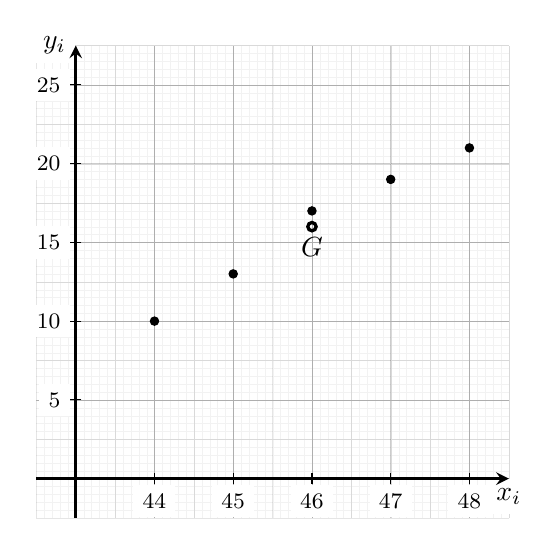
\begin{tikzpicture}[>=stealth,x=1.0cm,y=1.0cm,ybar,ycomb]
                                    \draw [xstep=0.1cm,ystep=0.1cm,opacity=.05,line width=.05]
                                          (-0.5,-0.5) grid (5.5,5.5);
                                    \draw [xstep=0.5cm,ystep=0.5cm,opacity=0.1,line width=0.1]
                                          (-0.5,-0.5) grid (5.5,5.5);
                                    \draw [xstep=1.0cm,ystep=1.0cm,opacity=0.2,line width=0.2]
                                          (-0.5,-0.5) grid (5.5,5.5);
                                    \draw[] (0,5.5) node[fill=white, left] {$y_i$};
                                    \draw[] (5.5,0) node[fill=white, below] {$x_i$};
                                    \draw[->,color=black, line width=1pt] (-0.5,0) -- (5.5,0);
                                    \foreach \x/\xtext in {1/44,2/45,3/46,4/47,5/48}
                                    \draw[shift={(\x,0)},color=black] (0pt,2pt) -- (0pt,-2pt) 
                                          node[below,fill=white] {\footnotesize $\xtext$};
                                    \draw[->,color=black, line width=1pt] (0,-0.5) -- (0,5.5);
                                    \foreach \y/\ytext in {1/5,2/10,3/15,4/20,5/25}
                                    \draw[shift={(0,\y)},color=black] (2pt,0pt) -- (-2pt,0pt) 
                                          node[left,fill=white] {\footnotesize $\ytext$};
                                    \foreach \x/\y in {1/2,2/2.6,3/3.4,4/3.8,5/4.2}
                                          \filldraw (\x,\y) circle (1.5pt);
                                    \draw[color = black, very thick] (3,3.2) circle (1.5pt) node[below] {$G$};
                              \end{tikzpicture}
                           \caption{Nuage de points et le point moyen $G$.}
                        \end{figure}
                  \end{ex}
            \end{defi}
            %
            \subsection{Ajustement affine}% (m\'ethode des moindres carr\'es)}
\index{Ajustement affine}
	                  Certaines s\'eries statistiques repr\'esentent des variables qui sont li\'ees.
                  Il est parfois possible de trouver une droite permettant d'approximer le nuage de points.
                  %
                  \subsubsection{Droite de r\'egression de $y$ en $x$}
\index{Droite de regression@Droite de r\'egression!de y en x@de $y$ en $x$}
	                        La droite de r\'egression obtenue par la m\'ethode des moindres carr\'es passe par le point moyen ;
                        ainsi, elle a une \'equation de la forme $y - \bar{y} = m (x - \bar{x})$ et le coefficient
                        directeur $m$ est \'egal \`a $\frac{\sigma_{xy}}{V(x)}$.
                  %
                  \subsubsection{Droite de r\'egression de $x$ en $y$}
\index{Droite de regression@Droite de r\'egression!de x en y@de $x$ en $y$}
                        Elle est donn\'ee par l'\'equation $x - \bar{x} = m' (y - \bar{y})$ et le coefficient
                        directeur $m'$ est \'egal \`a $\frac{\sigma_{xy}}{V(y)}$.
                  %
                  \subsubsection{Corr\'elation lin\'eaire}
\index{Correlation lineaire@Corr\'elation lin\'eaire}
                        Le coefficient de corr\'elation lin\'eaire sert \`a mesurer la relation entre les deux variables
                        $x$ et $y$.
                        Ce coefficient est donn\'e par \defbox{$\displaystyle{r = \frac{\sigma_{xy}}{\sigma_x \cdot \sigma_y}}$}.
                        \nota{
	                        Un coefficient de corr\'elation proche de $1$ ou $-1$ signifie que 
                        les deux variables sont << fortement corr\'el\'ees >>. \newline
	                        Comme $\sigma_x$, $\sigma_y$, $V(x)$ et $V(y)$ sont positifs, 
                        les signes de $m$, $m'$ et $r$ d\'ependent de celui de $\sigma_{xy}$.
                              \begin{align*}
                                    m\cdot m' & = \frac{\sigma_{xy}}{V(x)} \cdot \frac{\sigma_{xy}}{V(y)}        
                                                = \frac{(\sigma_{xy})^2}{\sigma_x^2 \cdot \sigma_y^2}            
                                                = \left( \frac{\sigma_{xy}}{\sigma_x \cdot \sigma_y} \right)^2   
                                                = r^2.
                              \end{align*}
                        }





















































\TCDLessonStyleOff
\clearpage
\providecommand{\cov}[2]{\mathrm{Cov}\left( #1 , #2 \right)}
\providecommand{\var}[1]{\mathrm{Var}\left( #1 \right)}
\section{Exercices}
      \begin{exo}
            Pour chacune des variables statistiques suivantes, dire si elle est qualitative ou quantitative ; 
            dans le cas d'une variable quantitative, dire si elle est discr\`ete ou continue.
            \begin{enumerate}
                  \item Couleur des yeux des \'el\`eves,
                  \item nombre d'enfants dans chaque foyer,
                  \item poids de nouveaux-n\'es dans un h\^opital,
                  \item nationalit\'es des participants \`a un championnat,
                  \item tailles des \'etudiants d'un lyc\'ee.
            \end{enumerate}
      \end{exo}
      %
      \begin{exo}
            Le tableau suivant donne la répartition selon le groupe sanguin de 60 individus pris au hasard.
            \begin{table}[H]
                  \centering
                        \begin{tabular}[b]{|c|c|c|c|c|}
                        \hline 
                        Groupes & O & A & B & AB \\ 
                        \hline 
                        Effectif & 10 & 22 & 17 & $n_{AB}$ \\ 
                        \hline 
                  \end{tabular}. 
            \end{table}
            \begin{enumerate}
                  \item Déterminer la variable statistique et son type.
                  \item Déterminer l’effectif des personnes ayant un groupe sanguin AB.
                  \item Repr\'esenter cette variable dans un diagramme en b\^aton
                        puis dans un diagramme en secteur.
            \end{enumerate}
      \end{exo}
      %
      \begin{exo}
	            On a relevé, pour un article particulier, le nombre d’articles vendus par jour dans un magasin.
	            Voici les nombres obtenus :
	            \begin{center}
	            \adjustbox{max width=\linewidth}{\begin{tabular}{lllllllllllllll}
                  $19$ & $24$ & $23$ & $20$ & $18$ & $19$ & $22$ & $25$ & $24$ & $23$ & $17$ & $21$ & $23$ & $19$ & $22$  \\
                  $19$ & $19$ & $21$ & $23$ & $20$ & $17$ & $21$ & $18$ & $21$ & $18$ & $22$ & $21$ & $20$ & $23$ & $20$  \\
                  $18$ & $19$ & $23$ & $22$ & $18$ & $19$ & $20$ & $20$ & $19$ & $20$ & $17$ & $19$ & $25$ & $26$ & $20$  \\
                  $23$ & $18$ & $20$ & $21$ & $21$ & $21$ & $22$ & $23$ & $22$ & $17$ & $16$ & $20$ & $22$ & $25$ & $20$  \\
	            \end{tabular}}
	            \end{center}
            %
            \begin{enumerate}
	                  \item Quelle est la variable \'etudi\'ee\,?
                  \item Dresser le tableau statistique repr\'esentant cette variable,
	                        en y indiquant les effectifs, la fr\'equence, la fr\'equence cumul\'ee ainsi que les effectifs cumul\'es.
                  \item Tracer le diagramme en b\^aton associ\'e \`a cette variable.
                  \item D\'eterminer le mode ainsi que la m\'ediane.
                  \item Calculer la moyenne arithm\'etique, la variance ainsi que l'\'ecart-type.
            \end{enumerate}
      \end{exo}
      %
      \begin{exo}
            Les moyennes g\'en\'erales des \'etudiants d'un lyc\'ee sont les suivantes : \newline
            \begin{tabular}[b]{rrrrrrrrrrrrrrr}
                  $9.46$ & $9.13$ & $13.61$ & $11.61$ & $9.06$ & $8.38$ & $10.64$ & $8.66$ & $14.56$ \\
                  $11.51$ & $10.96$ & $12.54$ & $10.00$ & $14.34$ & $13.17$ & $8.13$ & $9.01$ & $8.33$ \\
                  $6.82$ & $11.40$ & $9.43$ & $12.12$ & $10.16$ & $12.67$ & $6.55$ & $7.58$ & $5.72$ \\
                  $11.34$ & $12.88$ & $8.12$ & $8.79$ & $15.27$ & $8.26$ & $9.83$ & $8.33$ & $9.32$ \\
            \end{tabular}.
            %
            \begin{enumerate}
	                  \item Quelle est la variable \'etudi\'ee\,?
                  \item Dresser le tableau statistique repr\'esentant cette variable,
                        mettez-y les classes, les effectifs, la fr\'equence, la fr\'equence cumul\'ee ainsi que les effectifs cumul\'es.
                        (On prendra des classes d'amplitudes 2 en commen\c{c}ant par $[5,5 \ ; \ 7,5[$.
                  \item Tracer un histogramme associ\'e \`a cette variable.
                  \item D\'eterminer le mode ainsi que la m\'ediane.
                  \item Calculer la moyenne arithm\'etique, la variance ainsi que l'\'ecart-type.
            \end{enumerate}
      \end{exo}
      %
      \begin{exo}
            Un boulanger vend des pains qui doivent peser 200~g.
            Cependant, la perfection n'est pas de ce monde et les poids de son pain varient.
            Voici les poids de 60 pains pris au hasard :
            \begin{center}
            \adjustbox{max width=\linewidth}{%
            \begin{tabular}{llllllll}
                  $200.9$ & $198.8$ & $200.4$ & $199.5$ & $201.3$ & $200.8$ & $199.1$ & $202.8$ \\
                  $199.7$ & $200.9$ & $202.5$ & $200.9$ & $200.0$ & $200.3$ & $200.0$ & $198.8$ \\
                  $199.5$ & $199.6$ & $200.3$ & $198.3$ & $200.0$ & $201.4$ & $200.6$ & $200.0$ \\
                  $199.2$ & $199.7$ & $201.2$ & $200.2$ & $200.1$ & $199.2$ & $201.2$ & $200.5$ \\
                  $200.7$ & $198.8$ & $199.7$ & $198.4$ & $196.7$ & $198.6$ & $197.4$ & $201.1$ \\
                  $199.1$ & $201.5$ & $197.1$ & $200.3$ & $200.6$ & $200.7$ & $200.2$ & $199.9$ \\
                  $198.0$ & $202.9$ & $199.3$ & $199.2$ & $199.9$ & $201.7$ & $201.5$ & $198.4$ \\
            \end{tabular}%
            }
            \end{center}
            %
            \begin{enumerate}
	                  \item Quelle est la variable \'etudi\'ee\,?
                  \item Dresser le tableau statistique repr\'esentant cette variable,
                        mettez-y les classes, les effectifs, la fr\'equence, la fr\'equence cumul\'ee ainsi que les effectifs cumul\'es.
                        (On prendra des classes d'amplitudes 1~g en commen\c{c}ant par $[196 ; 197[$.
                  \item Tracer un histogramme associ\'e \`a cette variable.
                  \item D\'eterminer le mode ainsi que la m\'ediane.
                  \item Calculer la moyenne arithm\'etique, la variance ainsi que l'\'ecart-type.
            \end{enumerate}
      \end{exo}
      %
      \begin{exo}
            Une usine produit des pièces d'une machine. 
            Pour chaque pièce (individu), on dispose du coût de sa production (en milliers d'ariary) et 
            du temps nécessaire pour sa réalisation (en heures). 
            Le tableau ci-après (série statistique) donne cette répartition : \newline
            \begin{tabular}[b]{|c|c|c|c|c|c|}
                        \hline 
                  Individu & 1 & 2 & 3 & 4 & 5 \\ 
                        \hline 
                  Temps ($X$) mesur\'e en heures & 2 & 3 & 52 & 2 & 4 \\ 
                        \hline 
                  Co\^ut ($Y$) mesur\'e en milliers d'Ariary & 10 & 16 & 23 & 12 & 18 \\ 
                        \hline 
            \end{tabular}. \newline
            On rappelle les formules suivantes :
            \begin{itemize}
                  \item $\cov{X}{Y} 
                        = \displaystyle{\frac{1}{N} \sum_{i=1}^{n} \left[ (x_i - \bar{x}) (y_i - \bar{y} ) \right]}$,
                  \item $r = \frac{\cov{X}{Y}}{\sigma(X) \sigma(Y)}$,
                  \item Droite de corr\'elation :
                        $Y = \frac{\cov{X}{Y}}{\var{X}} \cdot \left( X - \bar{x} \right) + \bar{y}$.
            \end{itemize}
            
            \begin{enumerate}
                  \item Calculer la moyenne de la variable statistique $X$.
                  \item Calculer la moyenne de la variable statistique $Y$.
                  \item Calculer l'\'ecart-type de la variable statistique $X$.
                  \item Calculer l'\'ecart-type de la variable statistique $Y$.
                  \item Calculer la covariance des variables statistiques $X$ et $Y$.
                  \item En supposant qu'il existe une corr\'elation entre $X$ et $Y$, 
                        d\'eterminer cette droite de corr\'elation.
                  \item Calculer le coefficient de corr\'elation. Conclusion\,?
                  \item Une nouvelle pièce est réalisée en 6 heures. 
                        Estimer le coût de production de cette pièce en utilisant la droite de corrélation établie.
            \end{enumerate}
      \end{exo}
%%%%%%%%%%%%%%%%%%%%%%%%%%%%%%%%%%%%%%%%%%%%%%%%%%%%%%%%%%%%%%%%%%%%%%%%%
%%%%%%%%%%%%%%%%%%%%%%%%%%%%%%%%%%%%%%%%%%%%%%%%%%%%%%%%%%%%%%%%%%%%%%%%%














